\subsection{Charge density plots}
	We are using hydrogenic orbitals to structure the orbitals of our bigger atoms.

	\begin{tikzpicture}[domain=0:10, range = 0:6]
    % \draw[very thin,color=gray] (-0.1,-1.1) grid (3.9,3.9);
	    \draw[->] (-0.2,0) -- (10,0) node[below] {$r$};
	    \draw[->] (0,0) -- (0,4) node[left] {$|R(r)|^2$};
	    % \draw[color=red] plot[id=x, samples = 100, domain = 0:3] function{175*x**2*exp(-x/0.2)} 
	   	\draw[color=red] plot[id=exp, samples = 100, domain = 0:5] function{6*x**2*(2*exp(-x))**2} 
	        node[above] {$\psi_{S1}$};
	    \draw[color=blue] plot[id=sin, samples = 100] function{6*x**2*(1/(2*sqrt(2))*(2-x)*exp(-x/2))**2} 
	        node[above] {$\psi_{S2}$};
	    \draw[color=orange] plot[id=exp] function{6*x**2* ( 1/(2*sqrt(6)) * x  * exp(-x/2))**2} 
	        node[right] {$\psi_{P2}$};
	\end{tikzpicture}



	\subsubsection{Helium Atom}
		For the Helium atom we have ran simulations, with \(10^6\) Monte Carlo cycles, of several different trialfunctions and recorded the position of the electrons. We first did an experiment with the electrons being in a pure hydrogenlike wavefunction, then we ran an hydrogenlike wavefunction but optimized the \(\alpha \) value to get a better ground state energy then at last we also included a Pàde-Jastrow correlation factor to include the effects of the electron-electron repulsion. For the pure hydrogenic wavefunction we got $E = -2.757$ and $\sigma^2_* = 0.0030$, while with the optimized \(\alpha\) value we got $\alpha = 1.65$, $E = -2.843$ and $\sigma^2_* = 0.0027$, and lastly with the Pàde-Jastrow factor we got $\alpha = 1.843$, $\beta = 0.34$, $E = -2.887$, $\sigma^2_* = 0.0010$. Here $\sigma^2_*$ is the variance for the local energy between each particle move in the VMC, not the true variance, which is obtained through the blocking routine described in \cref{sec:blocking}. In figure \ref{fig:HeliumChargeDensity} we plots of the positions the electrons occupied during the simulations and we can see that for the pure hydrogenic wavefunction the electrons was generally closer to the nucleus than in the other two simulations. The ground-state energy improved and got closer to the reference value \ref{tab:energyReference1} as the wavefunction got more sophisticated as well as the variance decreasing. In the wavefunction the $\alpha$ parameter represents the electrical attraction of the nucleus on the electron, and is equal to the charge in a Hydrogen atom, in a real Helium atom the attraction felt is smaller than the charge of the nucleus since there is also an other electron that it feels. This is why we get a better simulation with a smaller \(\alpha\) value. For the Helium atom the effect of the correlation factor is not very pronounced, since the electrons can quite far away from each other, but it is still significant in the ground-state energy and the variance.
		\begin{figure}
				\centering 
				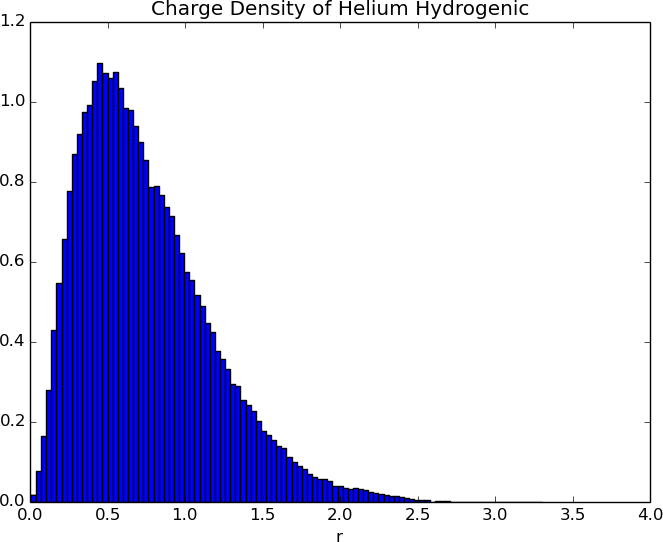
\includegraphics[width=0.32\linewidth]{../figures/used/ChargeDensityHeliumHydrogenic}
				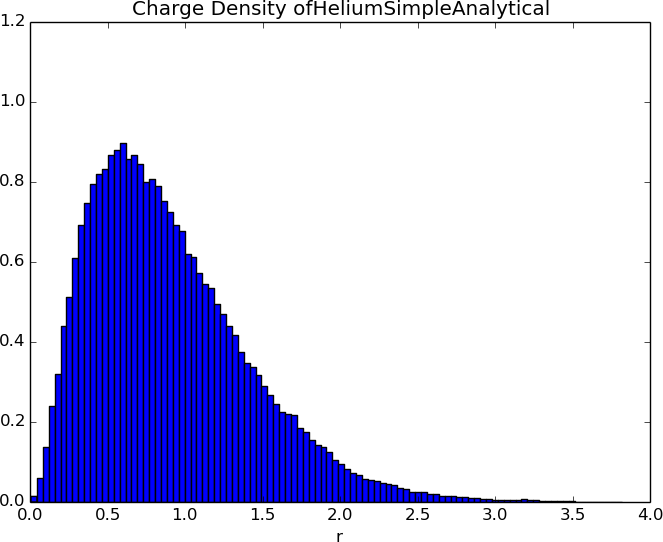
\includegraphics[width=0.32\linewidth]{../figures/used/ChargeDensityHeliumSimpleAnalytical}
				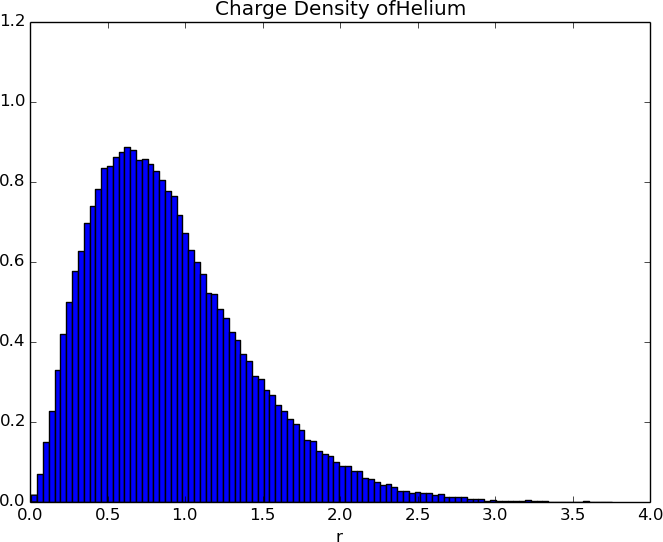
\includegraphics[width=0.32\linewidth]{../figures/used/ChargeDensityHelium_trimmed}
				\protect\caption{The electron-nucleus distance in an Helium atom simulated with different trialfunctions. From the left the plots represents pure hydrogenic wavefunctions ($\alpha = 2$, $E = -2.757$ and $\sigma^2_* = 0.0030$), hydrogenic wavefunctions with an optimized alpha ($\alpha = 1.65$, $E = -2.843$ and $\sigma^2_* = 0.0027$) and hydrogenic wavefunctions with a Jastrow factor and optimized parameters, ($\alpha = 1.843$, $\beta = 0.34$, $E = -2.887$, $\sigma^2_* = 0.0010$ ). The simulations were run with \(10^6\) Monte Carlo cycles.}
				\label{fig:HeliumChargeDensity}
		\end{figure}


	\subsubsection{Beryllium}
		% The charge density gives measure of how often the electrons occupies certain area in the Monte Carlo simulation, in figure \ref{fig:charge_density} the square of the norm of the distance is plotted.
		% On the Neon atom the electrons have a closer distribution to the center that is caused by the more electrically charged core of Neon compared to Beryllium.

		\begin{figure}
			\centering 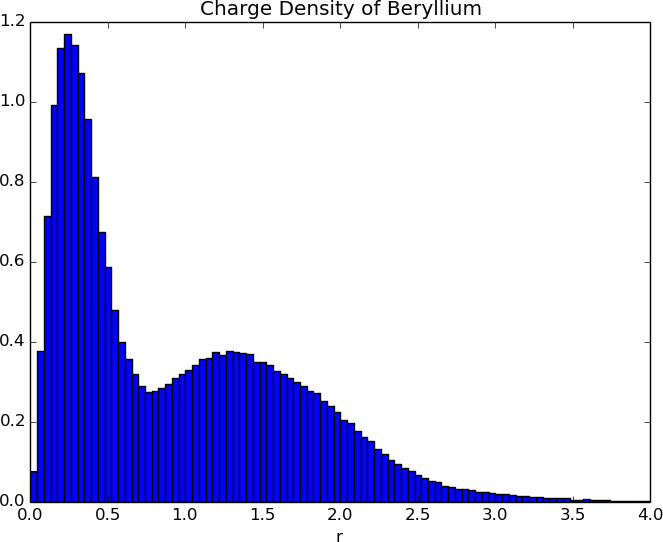
\includegraphics[width=0.45\linewidth]{../figures/used/ChargeDensityBerylliumSimple}
			\centering 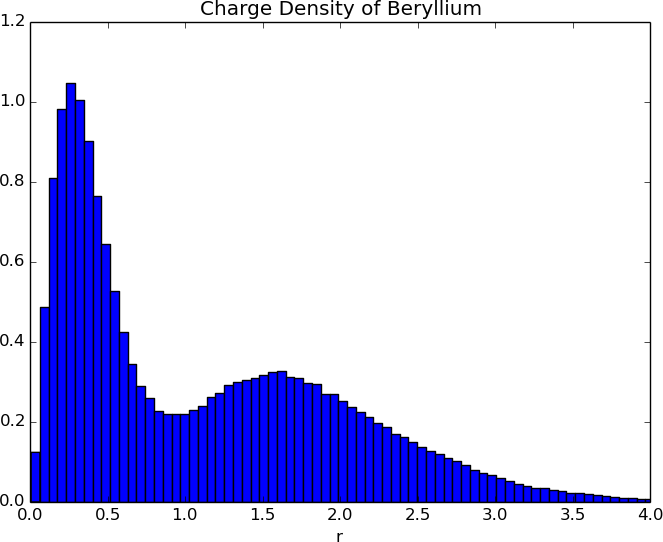
\includegraphics[width=0.45\linewidth]{../figures/used/ChargeDensityBeryllium}
			\protect\caption{Hydrogenic, $\alpha = 4$, $E = 13.710$, $\sigma^2_* = 0.0072$, Pàde-Jastrow, $\alpha = 4$, $\beta = 0.31$,  $E = 14.385$, $\sigma^2_* = 0.0029$}
			\label{fig:chargeDensityBeryllium}
		\end{figure}

		
	\subsubsection{Neon}
		\begin{figure}
			\centering 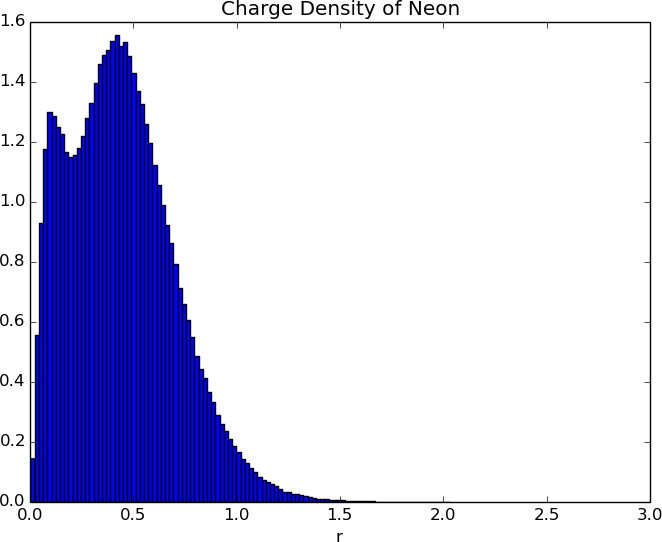
\includegraphics[width=0.45\linewidth]{../figures/used/ChargeDensityNeonSimple}
			\centering 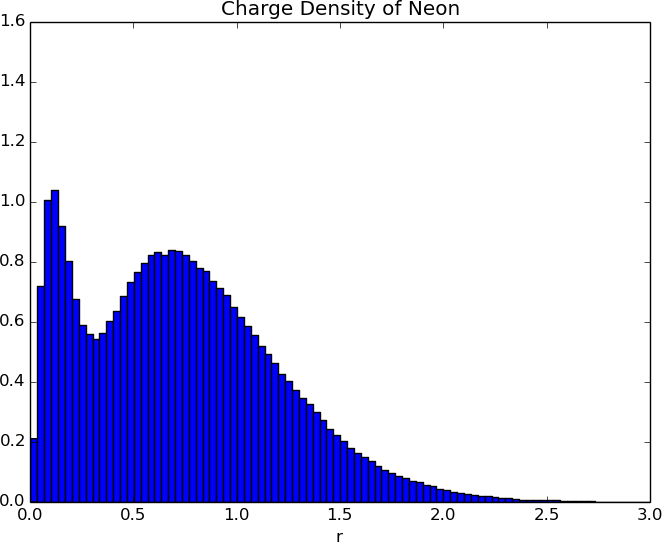
\includegraphics[width=0.45\linewidth]{../figures/used/ChargeDensityNeon}
			\protect\caption{Hydrogenic, $\alpha = 10.22$, $E = -110.301$, $\sigma^2_* = 0.0477$, Pàde-Jastrow, $\alpha = 10.22$, $\beta = 0.0.091$,  $E = -127.888$, $\sigma^2_* = 0.019$}
			\label{fig:chargeDensityNeon}
		\end{figure}